\documentclass[crop,tikz]{standalone}
\usepackage{circuitikz}
\ctikzset{bipoles/length=.8cm}
\tikzset{component/.style={draw,thick,circle,fill=white,minimum size =0.8cm,inner sep=0pt}}
\begin{document}
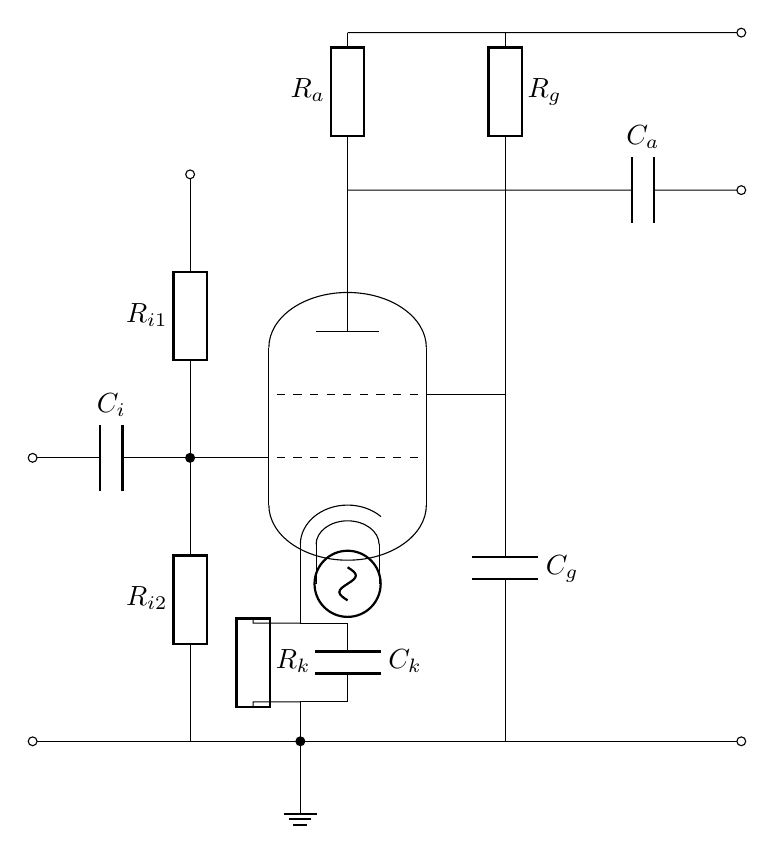
\begin{tikzpicture}
    \begin{scope}
        % корпус
        \draw (-1, -1) -- (-1, 1);
        \draw (1, -1) -- (1, 1);
        \draw (1, 1) arc (0:180:1 and 0.7);
        \draw (-1, -1) arc (180:360:1 and 0.7);
        % нагреватель
        \draw (-0.4, -2) -- (-0.4, -1.5);
        \draw (0.4, -2) -- (0.4, -1.5);
        \draw (0.4, -1.5) arc (0:180: 0.4 and 0.3);
        \draw (-0.4,-2) to[sV] (0.4, -2);
        % катод
        \draw (-0.6, -2.5) -- (-0.6, -1.5);
        \draw (-0.6, -1.5) arc (180:45: 0.6 and 0.5);
        % анод
        \draw (0, 2) -- (0, 1.2);
        \draw (0.4, 1.2) -- (-0.4, 1.2);
        % сетки
        \draw (-2, -0.4) -- (-1, -0.4);
        \draw[dashed](-0.9, -0.4) -- (0.9, -0.4);

        \draw[dashed](-0.9, 0.4) -- (0.9, 0.4);
        \draw (1, 0.4) -- (2, 0.4);
    \end{scope}

    \draw (0, 5) to[short,-o] (5, 5);
    \draw (2, 5) to[european,R=$R_g$] (2, 3.5) --  (2, 0.4) to[C=$C_g$] (2, -4);

    \draw (0, 2) -- (0,3.5) to[european,R=$R_a$] (0, 5);
    \draw(0, 3) -- (3, 3) to[C=$C_a$] (4.5,3) to[short,-o] (5,3);

    \draw (-0.6, -2.5) -- (0, -2.5) to[C=$C_k$] (0, -3.5) -- (-0.6, -3.5)
    -- (-0.6, -4) to[short, *-] (-0.6, -4.5) node[ground]{};
    \draw (-0.6, -2.5) -- (-1.2, -2.5) to[european, R=$R_k$] (-1.2, -3.5) --
    (-0.6, -3.5);

    \draw (-4, -4) to[short,o-o] (5, -4);
    \draw (-2, -4) to[european, R=$R_{i2}$] (-2, -0.4) to[european,
    R=$R_{i1}$,-o]
    (-2, 3.2);
    \draw (-4, -0.4) to[C=$C_i$,o-*] (-2,-0.4);
\end{tikzpicture}
\end{document}
